\section{Обзор}
В данном разделе представлен обзор предметной области:
общие сведения; способы реализации предметно-ориентированных
языков; процесс отображения пользовательских интерфейсов; существующие языки
программирования общего назначения, предоставляющие пользователям возможность декларативного описания пользовательских
интерфейсов с помощью предметно-ориентированных языков.

\subsection{Общие сведения}
\subsubsection{Завершающие лямбда-выражения}
\label{section:trailing-lambdas}
\textit{Завершающие лямбда-выражения} (от англ. \textit{trailing lambdas})
--- синтаксические возможности некоторых языков программирования,
позволяющие при вызове функции, последним формальным параметром которой
является другая функция, передать в качестве последнего
аргумента лямбда-выражение, вынесенное за пределы синтаксического контекста
остальных аргументов.

На листинге~\ref{lst:antlr-trailing-lambda} представлено упрощённое
синтаксическое правило передачи конечных лямбда-выражений, записанное
в нотации инструмента \name{ANTLR4}~\cite{antlr-homepage}.
\begin{lstlisting}[style=Antlr, caption=Синтаксис завершающих
лямбда-выражений, label={lst:antlr-trailing-lambda}]
trailingLambda
	: '{' parameters '->' returnType 'in' expressionList '}'
	;

functionCall
	: functionName arguments? trailingLambda?
	;
\end{lstlisting}
\subsubsection{Непрозрачные типы}
\label{section:opaque-types}
\textit{Непрозрачные типы} (от англ. \textit{opaque types})
--- механизм типовой системы языка программирования и его компилятора,
позволяющий функции или методу с непрозрачным типом возвращаемого значения
скрывать информацию типе возвращаемого значения. Вместо того, чтобы
указывать конкретный тип в качестве типа возвращаемого значения функции,
тип возвращаемого значения описывается в терминах интерфейсов, которым
он соответствует. В отличие от возврата значения, тип которого является
типом интерфейса, непрозрачные типы сохраняют идентичность ---
компилятор имеет доступ к информации о конкретном типе, в то время как
клиенты функции или метода его не имеют.
\subsubsection{\name{Accord}: спецификации}
\label{section:accord-specs}
Спецификации в языке \name{Accord} --- тип данных, являющийся именованным
множеством сигнатур методов. Тип данных $T$ называется соответствующим
спецификации $S$ тогда и только тогда, когда
$SM \subseteq TM$, где $SM$ --- множество сигнатур методов спецификации $S$,
$TM$ --- множество сигнатур методов типа $T$. Проверка на соответствие
объекта определённого типа той или иной спецификации происходит во время
выполнения программы за исключением случаев, когда данная проверка может
быть проведена во время компиляции исходного кода с использованием
статической информации о программе.

\subsection{Предметная область}
\subsubsection{Предметно-ориентированные языки}
\label{dsl-section}
Предметно-ориентированный язык (\textit{domain-specific language}, DSL) ---
это язык программирования с более высоким уровнем абстракции,
отражающий специфику решаемых с его помощью задач. Такой язык оперирует
понятиями и правилами из определенной предметной области~\cite{book-of-dsls}.

В отличие от языков программирования общего назначения, таких как \name{C},
\name{Python}, \name{Java}, предметно-ориентированные языки предоставляют
абстракции, адекватные решаемой проблеме, позволяя выражать решения,
написанные с их помощью, кратко и ёмко; причём в некоторых случаях
использование DSL не требует квалификации программиста.
В качестве примера DSL можно привести \name{SQL} ---  декларативный язык
программирования, применяемый для создания, модификации и управления данными в
реляционной базе данных.
Основным недостатком применения предметно-ориентированных языков является
стоимость их разработки, требующая экспертизы как в области разработки языков
программирования, так и в целевой предметной области.
Это является одной из причин того, что предметные языки редко применяются
для решения задач программной инженерии, в отличие от языков программирования
общего назначения.
Другой причиной отказа от обособленных предметных языков является тот факт,
что сочетание программной библиотеки и языка программирования общего
назначения может заменять DSL.
Программный интерфейс (\textit{Application Programming Interface},
API) библиотеки содержит специфичный для определённой
области словарь, образованный именами классов, методов и функций, доступный
всем пользователям языков программирования общего назначения, подключившим
библиотеку.
Однако, вышеприведённый подход проигрывает предметным языкам в следующих
аспектах~\cite{when-and-how-develop-dsl,dsl-spectrum-wile}:
\begin{itemize}
	\item устоявшаяся в области нотация, как правило, выходит за рамки
	ограниченных механизмов определения пользовательских операторов,
	предоставляемых языками общего назначения;
	\item абстракции определённой области не всегда могут быть
	просто отображены в конструкции языков общего назначения~\cite{dsl-traversal-transform};
	\item использование предметно-ориентированного языка сохраняет
	возможность анализа, верификации, оптимизации, параллелизации и
	трансформации в рамках конкретной области, что, в случае работы с
	исходным текстом языка программирования общего назначения, является
	более сложной задачей.
\end{itemize}

\subsubsection{Подходы к реализации предметно-ориентированных языков}
В последнее время всё больше исследований в области
предметно-ориен\-тированных языков направлены на категоризацию предметных
языков, а также выработку советов и лучших практик, отвечающих на вопросы
"когда и как?" создавать DSL для конкретной области~\cite{when-and-how-develop-dsl,study-on-preliminary-approaches-develop-dsl,spinellis-dsl-patterns}.
\paragraph{Препроцессинг}
DSL-конструкции транслируются в более низкоуровневый программный код
базового языка программирования общего назначения.
\begin{itemize}
	\item \textit{Макрокоманда}. Конструкции предметного языка представлены
	символьными именами, заменяемыми при обработке препроцессором на
	последовательность программных инструкций базового языка.
	\item \textit{Транспиляция}. Исходный код предметного языка
	транслируется в исходный код языка общего назначения.
	\item \textit{Лексическая обработка}. Трансформация предметного языка в
	язык общего назначения осуществляется на уровне лексем.
\end{itemize}

Преимуществом данного подхода является простота реализации DSL, поскольку
большая часть семантического анализа выполняется средствами базового языка.
В то же время, это является и недостатком данного подхода ввиду отсутствия
предметно-ориентированного статического анализа, оптимизаций и сообщений об ошибках.

\paragraph{Встраивание в базовый язык}
В данном подходе конструкции базового языка используются для построения
библиотеки предметно-ориен\-тированных операций. С помощью синтаксиса
базового языка задаётся диалект, максимально приближенный к определённой
предметной области.

Преимуществом данного подхода является полное переиспользование компилятора или интерпретатора базового языка для построения DSL. Основными недостатками
являются сообщения об ошибках, соответствующие спецификации базового языка,
и ограниченная синтаксическая выразительность, обусловленная
существующим синтаксисом базового языка.

\paragraph{Самостоятельный компилятор}
В данном подходе для создания DSL используются методы построения
компиляторов или интерпретаторов. В случае компилятора, конструкции
предметного языка транслируются во внутреннее представление компилятора, а
статический анализ производится над спецификацией DSL. В случае
интерпретатора, конструкции предметного языка распознаются и выполняются
в ходе цикла выборки-распознавания-исполнения (fetch-decode-execute cycle).

Преимуществами данного подхода являются приближенные к предметной
области синтаксис языка и сообщения об ошибках. Серьёзным недостатком
является необходимость создания нового компилятора или интерпретатора
предметного языка.

\paragraph{Компилятор компиляторов}
Данный подход схож с предыдущим за исключением того, что все или некоторые
стадии компиляции выполняются с использованием \textit{компилятора компиляторов} --- программы, воспринимающей синтаксическое или семантическое
описание языка программирования и генерирующей компилятор для этого языка.

Преимуществом подхода является снижение расходов на создание компилятора
предметного языка. Ограниченность итогового DSL возможностями используемого
компилятора компиляторов, а также сложность проработки предметного языка в
деталях, что может быть критично для достижения определённого уровня
производительности и близости сообщений об ошибках к предметной области,
составляют недостатки данного подхода.

\paragraph{Расширение существующего компилятора}
Компилятор языка программирования общего назначения расширяется
предметно-ориенти\-рованными правилами оптимизации и/или генерации кода.

В сравнении с предыдущим, данный подход менее трудоёмок из-за возможности
переиспользования частей существующего компилятора. Однако, стоит отметить,
что расширение существующего компилятора может оказаться сложной задачей,
для выполнения которой необходима поддержка расширений со стороны
компилятора языка общего назначения, а также минимизация пересечений
синтаксиса и семантики базового и предметного языков.

\paragraph{Использование готовых инструментов}
Существующие инструменты и нотации адаптируются под конкретную предметную
область. Примером такого подхода являются DSL, основанные на нотации
\name{XML}. В большинстве случаев предметные языки, полученные данным
способом, плохо подходят для их использования людьми в ручном режиме.

\subsubsection{Отображение пользовательского интерфейса}
\label{section:render-pipeline}
В данном разделе описан процесс обновления пользовательского интерфейса,
ставший де-факто стандартом для популярных современных средств разработки
мобильных приложений. Стоит отметить, что далее будут рассмотрены лишь базовые принципы построения и отображения интерфейсов, которых должно быть
достаточно для объяснения тех или иных оптимизационных решений, принятых в
данной работе.

Задачей отображения пользовательского интерфейса занимается
так называемый движок рендеринга или отрисовки (\textit{ren\-dering engine})
--- программное обеспечение, генерирующее изображение по модели.
Здесь \textit{модель} --- это описание любых объектов или явлений на строго
определённом языке или в виде структуры данных.

Процесс отрисовки кадра (рис. \ref{render-pipeline}) состоит из
последовательного построения нескольких древовидных структур, каждая из
которых является образом графического интерфейса, записанного пользователем
на некотором языке.
\begin{itemize}
	\item \textit{Дерево компонентов} --- древовидная структура данных,
	элементами которой являются	высокоуровневые компоненты интерфейса.
	Примером такого дерева может являться \name{DOM} (от англ.
	\textit{Document Object Model} --- объектная модель документа),
	использующийся в современных веб-браузерах.
	\item \textit{Дерево элементов} --- древовидная структура данных,
	изоморфная дереву компонентов, элементы которой могут быть
	использованы движком отрисовки для сравнения графических
	компонентов двух соседних кадров.
	\item \textit{Дерево рендеринга} --- древовидная структура данных,
	содержащая в себе только необходимые для непосредственно рендеринга
	элементы интерфейса. Говоря	о переходе между деревом элементов и деревом
	рендеринга как об отображении, можно сказать, что не все узлы дерева
	элементов имеют	свой образ в дереве рендеринга. Так же стоит отметить,
	что узлы дерева	рендеринга содержат в себе низкоуровневую информацию,
	такую как относительные координаты элемента в виртуальном пространстве
	движка отрисовки.
\end{itemize}

При отрисовке следующего кадра, движок рендеринга перерисовывает только
изменившиеся по сравнению с предыдущим кадром части интерфейса. Для этого,
между двумя соседними кадрами находится разница, которая и отправляется в
движок отрисовки. Нахождение этой разницы является одной из наиболее
ресурсоёмких операций во время выполнения приложения, поскольку она требует
создания нового дерева, обхода деревьев текущего и предыдущего кадров, а
также сравнения соответствующих элементов.

\begin{figure}[H]
\centering
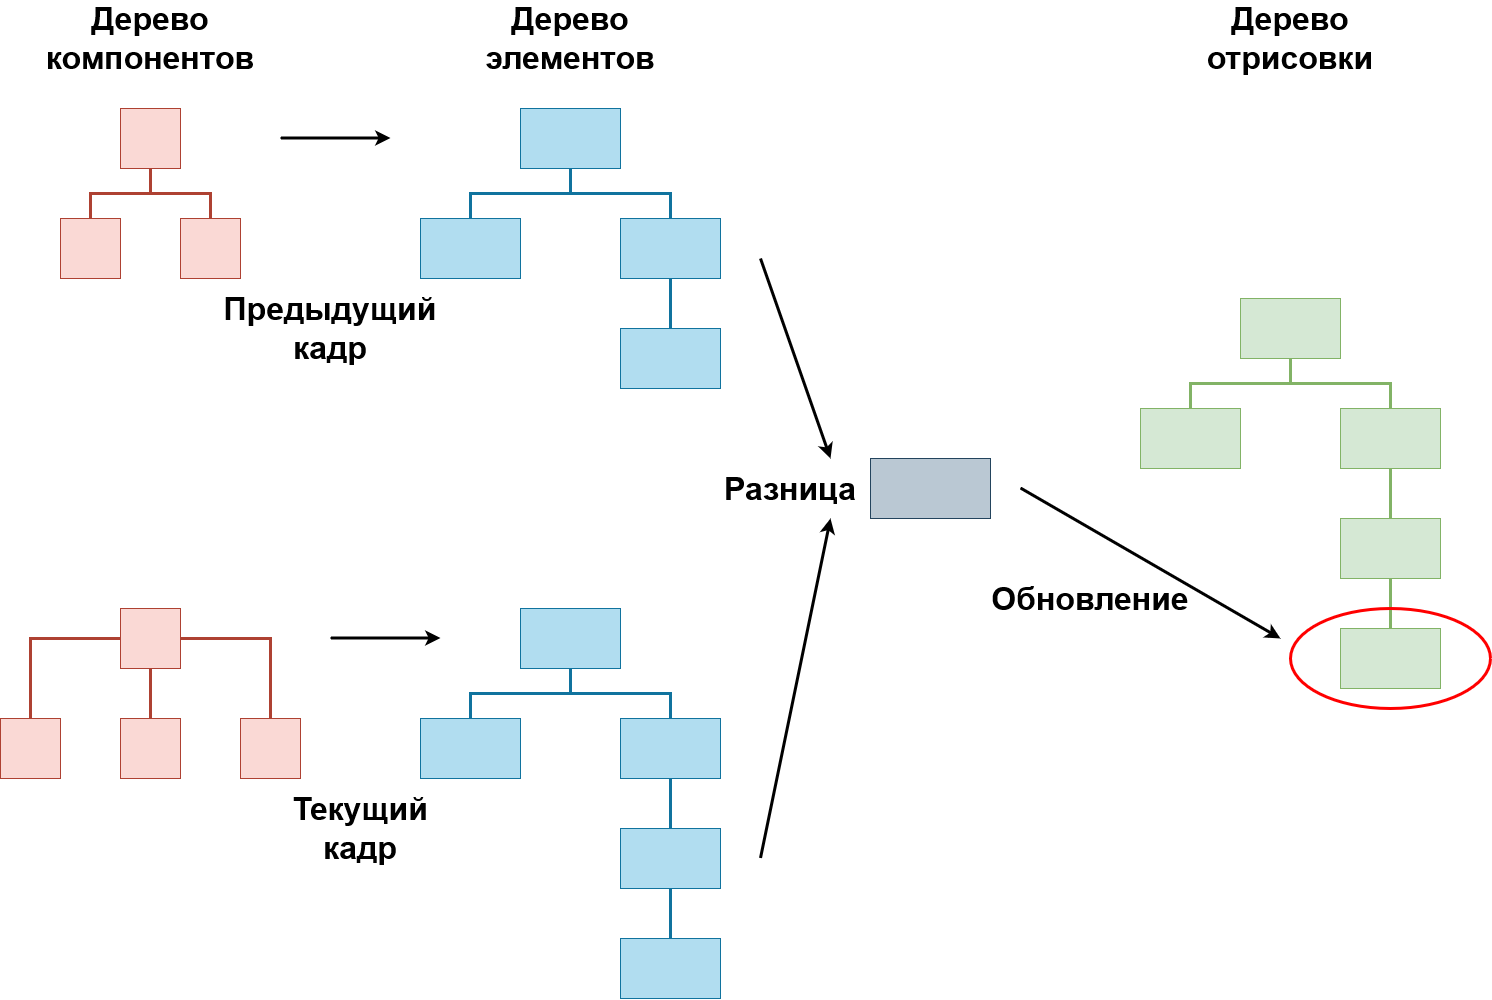
\includegraphics[width=\linewidth,height=0.9\linewidth,keepaspectratio]{resources/rendering-pipeline.png}
\caption{Процесс отображения пользовательского интерфейса}
\label{render-pipeline}
\end{figure}


% TODO: описание концепции состояния данных приложения

\subsection{Существующие решения}
\subsubsection*{Dart/Flutter}
\name{Flutter}~\cite{flutter-homepage} --- язык разработки
мобильных приложений, разрабатываемый компанией \name{Google}. По
сравнению с остальными решениями, данный язык в меньшей степени является
предметно-ориентированным, поскольку реализован в виде библиотеки
графических компонентов, создающей словарь предметной области, для языка
программирования общего назначения \name{Dart}~\cite{dart-homepage}.

На листинге \ref{lst:flutter-example} представлен пример приложения счётчика
количества нажатий на кнопку, написанное на языке \name{Dart}/\name{Flutter}.
Несмотря на то, что структура графического интерфейса описывается
декларативно, разработчику приходится сталкиваться с конструкциями,
традиционно присущими императивным языкам программирования:
\texttt{@override}, \texttt{return}. Более того, разделение реализации
графической компоненты на несколько связанных классов накладывает
определённые ограничения на минимальную квалификацию разработчика
графического интерфейса приложения, требуя от него наличия базовых навыков
программирования.
\begin{lstlisting}[language=Swift,caption=Счётчик нажатия кнопки на языке
\name{Dart}/\name{Flutter},label={lst:flutter-example}]
import '...'

class CounterApp extends StatelessWidget {
    @override
    Widget build(BuildContext context) {
        return MaterialApp(
            home: Counter(someCondition),
        );
    }
}

class Counter extends StatefulWidget {
    final bool condition;
    const Counter(this.condition);
    
    @override
    _CounterState createState() => _CounterState();
}

class _CounterState extends State<Counter> {
    int _counter = 0;
    
    void _incrementCounter() {
        setState(
            () { _counter++; }
        );
    }
    
    @override
    Widget build(BuildContext context) {
        return Column(
            children: <Widget>[
                Text("Current count: $_counter"),
                TextButton(
                    onPressed: _incrementCounter,
                    child: Text("Click on me!")
                ),
                widget.condition ?
                    Image.asset("assets/images/image.png") :
                    Text("Text Component")
            ]
        )
    }
}
\end{lstlisting}

Отрисовка графического интерфейса средством разработки мобильных
приложений \name{Dart}/\name{Flutter} осуществляется по классическому
алгоритму, описанному в главе~\ref{section:render-pipeline} за исключением
некоторых оптимизаций, направленных на уменьшение количества графических
компонентов, отслеживание изменений и перерисовку которых необходимо
выполнять во время исполнения приложения при каждой смене кадра. Так,
выполняя обход дерева элементов нового кадра и находя разницу между ним
и подобным деревом предыдущего кадра, проверка изменения некоторых
графических компонентов может быть опущена при условии выполнения
определённых условий, например:
\begin{itemize}
	\item соответствие динамического типа проверяемой графической компоненты
	некоторому типу, гарантирующему неизменяемость данной компоненты
	во время исполнения программы;
	\item наличие у потенциально изменяемой во время исполнения программы
	графической компоненты выставленного атрибута, указывающего
	на использование в данной компоненте неизменяемых данных (прим.:
	компонента \texttt{Text}, созданная при помощи строкового литерала).
\end{itemize}

\subsubsection*{Kotlin UI DSL}

\subsubsection*{React Native}

\subsubsection*{Swift/SwiftUI}
\name{SwiftUI}~\cite{swiftui-homepage} --- язык разработки мобильных
приложений, разрабатываемый компанией \name{Apple}. Данный
предметно-ориентированный язык реализован методом встраивания в базовый
язык, которым, в данном случае, является язык программирования общего
назначения \name{Swift}~\cite{swift-homepage}. В отличие от языка
\name{Swift}, являющегося открытым и свободным программным обеспечением,
исходный код и спецификация \name{SwiftUI} являются проприетарными и
закрытыми, что не позволяет провести полноценный анализ данного решения.
При этом, на основе наблюдаемого поведения программ, написанных на языке
\name{SwiftUI}, и доступной документации можно сделать некоторые выводы о
реализации \name{SwiftUI}.

Графический интерфейс приложений на языке \name{SwiftUI}
описывается декларативно:
\begin{lstlisting}[language=Swift,caption=Счётчик нажатия кнопки на языке
\name{SwiftUI},label={lst:swiftui-example}]
struct ContentView : View {
    var condition: bool
    @State var count: Int = 0
	
    var body: some View {
        VStack {
            Text("Current count: \(count)")
            Button(action: {
                self.count += 1
            }) {
                Text("Click on me!")
            }
            if condition {
                Image("path/to/image")
            } else {
                Text("text component")
            }
        }
    }
}
\end{lstlisting}
Каждый компонент графического интерфейса, описываемый пользователем, должен
явно указывать своё соответствие специальному
протоколу~\cite{swift-protocols-doc} \name{View}. Согласно этому протоколу,
тип, соответствующий ему, обязан иметь поле \name{body} соответствующего
протоколу \name{View} типа. На языке \name{Swift} данный
протокол может быть описать следующим образом:
\begin{lstlisting}[language=Swift, caption=Реализация протокола \name{View}
на языке \name{Swift}]
protocol View {
    associatedtype Body: View
    var body: Self.Body { get }
}
\end{lstlisting}

Для достижения декларативности, представленной на листинге
\ref{lst:swiftui-example}, разработчикам языка \name{Swift} потребовалось
расширить его спецификацию следующими нововведениями:
\begin{itemize}
	\item завершающие лямбда-выражения~\ref{section:trailing-lambdas};
	\item непрозрачные типы~\ref{section:opaque-types};
	\item неявный возврат значений из функций, состоящих из единственного
	выражения возврата результата.
\end{itemize}

Важной особенностью \name{SwiftUI} является высокая степень использования
информации, доступной во время компиляции программы, для оптимизации
процесса отображения пользовательского интерфейса. Во время компиляции
приложения для каждой пользовательской графической компоненты выводится
её статический тип. Так, графическая компонента, представленная на листинге
\ref{lst:swiftui-example}, имеет следующий статический тип данных:\newline
\texttt{VStack<Text, Button<Text>, \_ConditionalContent<Image, Text>>}.
Данный тип не будет изменён во время выполнения программы, что позволяет
избежать ресурсоёмкого шага алгоритма отрисовки графического интерфейса
--- нахождения разницы между деревьями элементов текущего и предыдущего
кадров: компилятор имеет информацию о том, какие графические компоненты
могут быть изменены во время исполнения программы, а также о их смещении
внутри структуры, которой представлен пользовательский интерфейс.


%\subsection{Вывод}
